\documentclass[10pt,aspectratio=169,serif]{beamer}

\usepackage[fontset=none, scheme=plain]{ctex}
\IfFontExistsTF{Songti SC}{%
	\setCJKmainfont{Songti SC}[AutoFakeSlant=0.2]%
	\setCJKsansfont{Songti SC}[AutoFakeSlant=0.2]%
}{%
	\setCJKmainfont{FandolSong-Regular}[Extension=.otf,BoldFont=FandolSong-Bold,AutoFakeSlant=0.2]%
	\setCJKsansfont{FandolSong-Regular}[Extension=.otf,BoldFont=FandolSong-Bold]%
}
\usepackage{amsmath,amssymb,graphicx,tikz,booktabs,multicol,calligra}
\usepackage{pgfplots}
\pgfplotsset{compat=1.18}
\usepackage{tcolorbox}
\tcbuselibrary{skins}
\usepackage{XyygU}
\usepackage{caption}
\captionsetup[figure]{name=图,labelsep=period}

\usetikzlibrary{arrows.meta,positioning,calc}

\setlength{\abovedisplayskip}{0pt plus 2pt minus 2pt}
\setlength{\belowdisplayskip}{0pt plus 2pt minus 2pt}

\title[习题2.2]{习题2.2 基本不等式}
\subtitle{复习巩固 \& 综合运用 \& 拓广探索}
\author{}
\institute{}
\date{2026-10-16}

\begin{document}

\begin{frame}
  \titlepage
\end{frame}

% ========== 第1题 ==========
\begin{frame}[t]{第1题：凑项求最值}
\textbf{1.}
\begin{enumerate}[(1)]
  \item 已知 $x>1$，求 $x+\dfrac{1}{x-1}$ 的最小值；
  \item 求 $\sqrt{x(10-x)}$ 的最大值。
\end{enumerate}
\end{frame}

\begin{frame}[t]{第1题 解答}
\begin{tcolorbox}[colback=orange!10,colframe=orange,title=\textbf{解}]
\textbf{(1)} 因为 $x>1$，所以 $x-1>0$。凑项：
\[
x+\frac{1}{x-1}=(x-1)+\frac{1}{x-1}+1.
\]
由基本不等式（积定和最小）：
\[
(x-1)+\frac{1}{x-1}\ge 2\sqrt{(x-1)\cdot\frac{1}{x-1}}=2.
\]
等号当 $x-1=\dfrac{1}{x-1}$，即 $(x-1)^2=1$，$x=2$（$x>1$）时成立。

故最小值为 $2+1=\alert{3}$（在 $x=2$ 时取得）。

\vspace{0.5em}
\textbf{(2)} 要有意义需 $x(10-x)\ge 0$，即 $0\le x\le 10$，此时 $x\ge 0,\ 10-x\ge 0$。
\[
x(10-x)\le \left(\frac{x+(10-x)}{2}\right)^2=25.
\]
等号当 $x=10-x$，即 $x=5$ 时成立。故 $\sqrt{x(10-x)}\le\sqrt{25}=5$，最大值为 $\alert{5}$。
\end{tcolorbox}
\end{frame}

% ========== 第2题 ==========
\begin{frame}[t]{第2题：和定积大·积定和小}
\textbf{2.}
\begin{enumerate}[(1)]
  \item 把 $36$ 写成两个正数的积，当这两个正数取什么值时，它们的和最小？
  \item 把 $18$ 写成两个正数的和，当这两个正数取什么值时，它们的积最大？
\end{enumerate}
\end{frame}

\begin{frame}[t]{第2题 解答}
\begin{tcolorbox}[colback=orange!10,colframe=orange,title=\textbf{解}]
\textbf{(1)} 设两正数为 $a,\ b$，则 $ab=36$（定值）。由基本不等式：
\[
a+b\ge 2\sqrt{ab}=2\sqrt{36}=12.
\]
等号当 $a=b$ 时成立。由 $ab=36$ 得 $a=b=6$。

故当两正数均为 $\alert{6}$ 时，和最小，最小值为 $\alert{12}$。

\vspace{0.5em}
\textbf{(2)} 设两正数为 $a,\ b$，则 $a+b=18$（定值）。由基本不等式：
\[
ab\le \left(\frac{a+b}{2}\right)^2=\left(\frac{18}{2}\right)^2=81.
\]
等号当 $a=b=9$ 时成立。

故当两正数均为 $\alert{9}$ 时，积最大，最大值为 $\alert{81}$。
\end{tcolorbox}
\end{frame}

% ========== 第3题 ==========
\begin{frame}[t]{第3题：房屋总造价最低}
\textbf{3.} 某公司建造一间背面靠墙的房屋，地面面积为 $48\ \mathrm{m^2}$，房屋正面每平方米的造价为 $1200$ 元，房屋侧面每平方米的造价为 $800$ 元，屋顶的造价为 $5800$ 元。如果墙高为 $3\ \mathrm{m}$，且不计房屋背面和地面的费用，那么怎样设计房屋能使总造价最低？最低总造价是多少？
\end{frame}

\begin{frame}[t]{第3题 解答}
\begin{tcolorbox}[colback=orange!10,colframe=orange,title=\textbf{解}]
设房屋正面长为 $x\ \mathrm{m}$，侧面长为 $y\ \mathrm{m}$。由地面面积：
\[
xy=48.
\]
墙高 $3\,\mathrm{m}$。正面造价：$1200\cdot 3x=3600x$；两个侧面造价：$2\times 800\cdot 3y=4800y$；屋顶 $5800$ 元。总造价：
\[
z=3600x+4800y+5800=1200(3x+4y)+5800.
\]

注意到 $(3x)(4y)=12xy=576$（定值），由基本不等式：
\[
3x+4y\ge 2\sqrt{(3x)(4y)}=2\sqrt{576}=48.
\]
等号当 $3x=4y=24$，即 $x=8,\ y=6$ 时成立（检验 $xy=48$）。

此时 $z_{\min}=1200\times 48+5800=\alert{63400}$ 元。

\vspace{0.3em}
故设计正面长 $\alert{8\,\mathrm{m}}$、侧面长 $\alert{6\,\mathrm{m}}$ 时总造价最低，为 $\alert{63400}$ 元。
\end{tcolorbox}
\end{frame}

% ========== 第4题 ==========
\begin{frame}[t]{第4题：连乘不等式}
\textbf{4.} 已知 $x,\ y,\ z$ 都是正数，求证：
\[
(x+y)(y+z)(z+x)\ge 8xyz.
\]
\end{frame}

\begin{frame}[t]{第4题 解答}
\begin{tcolorbox}[colback=orange!10,colframe=orange,title=\textbf{证明}]
因为 $x,\ y,\ z$ 均为正数，由基本不等式：
\[
x+y\ge 2\sqrt{xy},\qquad
y+z\ge 2\sqrt{yz},\qquad
z+x\ge 2\sqrt{zx}.
\]

三式两边均为正，分别相乘：
\begin{align*}
(x+y)(y+z)(z+x)
&\ge 2\sqrt{xy}\cdot 2\sqrt{yz}\cdot 2\sqrt{zx}\\
&=8\sqrt{x^2y^2z^2}\\
&=8xyz.
\end{align*}

当且仅当 $x=y=z$ 时，三个等号同时成立。

故 \alert{$(x+y)(y+z)(z+x)\ge 8xyz$}。
\end{tcolorbox}
\end{frame}

% ========== 第5题 ==========
\begin{frame}[t]{第5题：求最大值}
\textbf{5.} 已知 $x>0$，求证：$2-3x-\dfrac{4}{x}$ 的最大值是 $2-4\sqrt{3}$。
\end{frame}

\begin{frame}[t]{第5题 解答}
\begin{tcolorbox}[colback=orange!10,colframe=orange,title=\textbf{证明}]
因为 $x>0$，所以 $3x>0$，$\dfrac{4}{x}>0$。由基本不等式：
\[
3x+\frac{4}{x}\ge 2\sqrt{3x\cdot\frac{4}{x}}=2\sqrt{12}=4\sqrt{3}.
\]

两边乘 $-1$（反向）：
\[
-\left(3x+\frac{4}{x}\right)\le -4\sqrt{3}.
\]

两边加 $2$：
\[
2-3x-\frac{4}{x}\le 2-4\sqrt{3}.
\]

等号当 $3x=\dfrac{4}{x}$，即 $x^2=\dfrac{4}{3}$，$x=\dfrac{2}{\sqrt{3}}>0$ 时成立。

故 $2-3x-\dfrac{4}{x}$ 的最大值为 \alert{$2-4\sqrt{3}$}。
\end{tcolorbox}
\end{frame}

% ========== 第6题 ==========
\begin{frame}[t]{第6题：仓库选址}
\textbf{6.} 一家货物公司计划租地建造仓库储存货物，经过市场调查了解到下列信息：每月土地占地费 $y_1$（单位：万元）与仓库到车站的距离 $x$（单位：$\mathrm{km}$）成反比，每月库存货物费 $y_2$（单位：万元）与 $x$ 成正比；若在距离车站 $10\,\mathrm{km}$ 处建仓库，则 $y_1$ 和 $y_2$ 分别为 $2$ 万元和 $8$ 万元。这家公司应该把仓库建在距离车站多少千米处，才能使两项费用之和最小？
\end{frame}

\begin{frame}[t]{第6题 解答}
\begin{tcolorbox}[colback=orange!10,colframe=orange,title=\textbf{解}]
设 $y_1=\dfrac{k_1}{x}$，$y_2=k_2 x$。代入 $x=10$ 时 $y_1=2,\ y_2=8$：
\[
2=\frac{k_1}{10}\Rightarrow k_1=20;\qquad 8=10k_2\Rightarrow k_2=0.8.
\]
故 $y_1=\dfrac{20}{x}$，$y_2=0.8x$。两项费用之和：
\[
y=y_1+y_2=\frac{20}{x}+0.8x\quad (x>0).
\]

由基本不等式（积定和最小）：
\[
\frac{20}{x}+0.8x\ge 2\sqrt{\frac{20}{x}\cdot 0.8x}=2\sqrt{16}=8.
\]
等号当 $\dfrac{20}{x}=0.8x$，即 $x^2=25$，$x=5$ 时成立。

\vspace{0.3em}
故仓库应建在距离车站 $\alert{5\,\mathrm{km}}$ 处，两项费用之和最小，为 $\alert{8}$ 万元。
\end{tcolorbox}
\end{frame}

% ========== 第7题 ==========
\begin{frame}[t]{第7题：两臂不等的天平}
\textbf{7.} 一家商店使用一架两臂不等长的天平称黄金。一位顾客到店里购买 $10\,\mathrm{g}$ 黄金，售货员先将 $5\,\mathrm{g}$ 的砝码放在天平左盘中，取出一些黄金放在天平右盘中使天平平衡；再将 $5\,\mathrm{g}$ 的砝码放在天平右盘中，再取出一些黄金放在天平左盘中使天平平衡；最后将两次称得的黄金交给顾客。你认为顾客购得的黄金是小于 $10\,\mathrm{g}$，等于 $10\,\mathrm{g}$，还是大于 $10\,\mathrm{g}$？为什么？
\end{frame}

\begin{frame}[t]{第7题 解答}
\begin{tcolorbox}[colback=orange!10,colframe=orange,title=\textbf{解}]
设天平左臂长为 $l_1$，右臂长为 $l_2$（$l_1\ne l_2$），第一次称得黄金 $m_1$，第二次 $m_2$。

\textbf{第一次：} 砝码 $5\,\mathrm{g}$ 在左盘，黄金 $m_1$ 在右盘：
\[
5l_1=m_1l_2 \;\Rightarrow\; m_1=\frac{5l_1}{l_2}.
\]

\textbf{第二次：} 砝码 $5\,\mathrm{g}$ 在右盘，黄金 $m_2$ 在左盘：
\[
m_2l_1=5l_2 \;\Rightarrow\; m_2=\frac{5l_2}{l_1}.
\]

总黄金：
\[
m_1+m_2=5\left(\frac{l_1}{l_2}+\frac{l_2}{l_1}\right)\ge 5\cdot 2\sqrt{\frac{l_1}{l_2}\cdot\frac{l_2}{l_1}}=10.
\]
等号当 $\dfrac{l_1}{l_2}=\dfrac{l_2}{l_1}$，即 $l_1=l_2$ 时成立。但两臂不等，故严格大于。

\vspace{0.3em}
所以顾客购得的黄金 \alert{大于 $10\,\mathrm{g}$}。
\end{tcolorbox}
\end{frame}

% ========== 第8题 ==========
\begin{frame}[t]{第8题：矩形折叠求最大面积}
\textbf{8.} 设矩形 $ABCD$（$AB>AD$）的周长为 $24\,\mathrm{cm}$，把 $\triangle ABC$ 沿 $AC$ 向 $\triangle ADC$ 折叠，$AB$ 折过去后交 $DC$ 于点 $P$。设 $AB=x\,\mathrm{cm}$，求 $\triangle ADP$ 的最大面积及相应 $x$ 的值。
\end{frame}

\begin{frame}[t]{第8题 配图}
\begin{center}
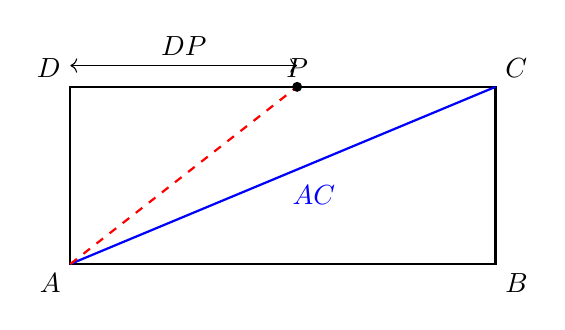
\begin{tikzpicture}[scale=0.9]
  % 矩形
  \draw[thick] (0,0) rectangle (6,2.5);
  \node[below left] at (0,0) {$A$};
  \node[below right] at (6,0) {$B$};
  \node[above right] at (6,2.5) {$C$};
  \node[above left] at (0,2.5) {$D$};
  % 对角线 AC
  \draw[thick,blue] (0,0) -- (6,2.5);
  \node[below right,blue] at (3,1.25) {$AC$};
  % 折叠后 AB' 交 DC 于 P
  \draw[thick,red,dashed] (0,0) -- (3.2,2.5);
  \fill[black] (3.2,2.5) circle (2pt);
  \node[above] at (3.2,2.5) {$P$};
  % DP 标注
  \draw[<->] (0,2.8) -- (3.2,2.8);
  \node[above] at (1.6,2.8) {$DP$};
\end{tikzpicture}
\end{center}
\end{frame}

\begin{frame}[t]{第8题 解答：建立关系}
\begin{tcolorbox}[colback=orange!10,colframe=orange,title=\textbf{解}]
设 $AB=x$，则 $AD=\dfrac{24-2x}{2}=12-x$（由 $AB>AD$ 知 $6<x<12$）。

折叠后 $\triangle ABC\cong\triangle AB'C$，故 $\angle BAC=\angle PAC$。

又矩形中 $AB\parallel DC$，内错角相等 $\angle BAC=\angle PCA$，所以 $\angle PAC=\angle PCA$，即 $\triangle PAC$ 为等腰三角形：
\[
PA=PC.
\]

设 $DP=p$，则 $PC=DC-DP=x-p$，故 $PA=x-p$。在 $\mathrm{Rt}\triangle ADP$ 中：
\[
PA^2=AD^2+DP^2.
\]
代入：
\[
(x-p)^2=(12-x)^2+p^2.
\]
展开：$x^2-2xp+p^2=(12-x)^2+p^2$，解得
\[
p=\frac{x^2-(12-x)^2}{2x}=\frac{24x-144}{2x}=\frac{12(x-6)}{x}.
\]
\end{tcolorbox}
\end{frame}

\begin{frame}[t]{第8题 解答：求最大值}
\begin{tcolorbox}[colback=orange!10,colframe=orange,title=\textbf{解 续}]
$\triangle ADP$ 为直角三角形（$\angle D=90^\circ$），其面积：
\[
S=\frac{1}{2}\cdot DP\cdot AD=\frac{1}{2}\cdot\frac{12(x-6)}{x}\cdot(12-x).
\]
化简：
\[
S=\frac{6(x-6)(12-x)}{x}=6\left(18-x-\frac{72}{x}\right).
\]

要使 $S$ 最大，只需使 $x+\dfrac{72}{x}$ 最小。因为 $x>0$，由基本不等式：
\[
x+\frac{72}{x}\ge 2\sqrt{x\cdot\frac{72}{x}}=12\sqrt{2}.
\]
等号当 $x=\dfrac{72}{x}$，即 $x^2=72$，$x=6\sqrt{2}$（满足 $6<x<12$）时成立。

此时
\[
S_{\max}=6(18-12\sqrt{2})=108-72\sqrt{2}\ \mathrm{cm^2}.
\]

\vspace{0.3em}
故当 $x=\alert{6\sqrt{2}\,\mathrm{cm}}$ 时，$\triangle ADP$ 面积最大，最大值为 $\alert{108-72\sqrt{2}\,\mathrm{cm^2}}$。
\end{tcolorbox}
\end{frame}

\begin{frame}[c]
  \begin{center}
    {\Huge\calligra Thanks!}
  \end{center}
\end{frame}

\end{document}
